% Created with jtex v.1.0.4
\documentclass{article}
\usepackage{arxiv}

\usepackage[utf8]{inputenc} % allow utf-8 input
\usepackage[T1]{fontenc}    % use 8-bit T1 fonts
\usepackage{hyperref}       % hyperlinks
\usepackage{url}            % simple URL typesetting
\usepackage{datetime}       % show dates in the title block
\usepackage{booktabs}       % professional-quality tables
\usepackage{amsfonts}       % blackboard math symbols
\usepackage{nicefrac}       % compact symbols for 1/2, etc.
\usepackage{microtype}      % microtypography
\usepackage{graphicx}
\usepackage{natbib}
\usepackage{doi}
\usepackage{xcolor}

%%%%%%%%%%%%%%%%%%%%%%%%%%%%%%%%%%%%%%%%%%%%%%%%%%
%%%%%%%%%%%%%%%%%%%%  imports  %%%%%%%%%%%%%%%%%%%
\usepackage{amsmath}
%%%%%%%%%%%%%%%%%%%%%%%%%%%%%%%%%%%%%%%%%%%%%%%%%%

\hypersetup{colorlinks = true,
linkcolor = purple,
urlcolor  = blue,
citecolor = cyan,
anchorcolor = black}

\title{The attractor states of the functional brain connectome}

\newdate{articleDate}{10}{8}{2023}
\date{\displaydate{articleDate}}

\makeatletter
\let\@fnsymbol\@arabic
\makeatother

\author{Robert Englert\\
Department of Diagnostic and Interventional Radiology and Neuroradiology,  University Medicine Essen, Germany\\\AND
Balint Kincses\\
Department of Neurology, University Medicine Essen, Germany\\\AND
Raviteja Kotikalapudi\\
Department of Neurology, University Medicine Essen, Germany\\\AND
Giuseppe Gallitto\\
Department of Neurology, University Medicine Essen, Germany\\\AND
Jialin Li\\
Department of Neurology, University Medicine Essen, Germany\\Max Planck School of Cognition, Leipzig, Germany\\\AND
Kevin Hoffschlag\\
Department of Neurology, University Medicine Essen, Germany\\\AND
Choong-Wan Woo\\
Center for Neuroscience Imaging Research, Institute for Basic Science, Suwon, South Korea\\Department of Biomedical Engineering, Sungkyunkwan University, Suwon, South Korea\\\AND
Tor D. Wager\\
Department of Psychological and Brain Sciences, Dartmouth College, Hanover, NH, USA\\\AND
Dagmar Timmann\\
Department of Neurology, University Medicine Essen, Germany\\Center for Translational Neuro- and Behavioral Sciences (C-TNBS), University Medicine Essen, Germany\\\AND
Ulrike Bingel\\
Department of Neurology, University Medicine Essen, Germany\\Center for Translational Neuro- and Behavioral Sciences (C-TNBS), University Medicine Essen, Germany\\\AND
\href{https://orcid.org/0000-0002-2942-0821}{
\includegraphics[scale=0.06]{orcid.pdf}}\hspace{1mm}Tamas Spisak\footnotemark[1]\\
Department of Diagnostic and Interventional Radiology and Neuroradiology,  University Medicine Essen, Germany\\Center for Translational Neuro- and Behavioral Sciences (C-TNBS), University Medicine Essen, Germany\\}

% Uncomment to override  the `A preprint' in the header
\renewcommand{\headeright}{Preprint}
\renewcommand{\undertitle}{}
\renewcommand{\shorttitle}{ConnAttractor Preprint}

%% Add PDF metadata to help others organize their library
%% Once the PDF is generated, you can check the metadata with
%% $ pdfinfo template.pdf
\hypersetup{
pdftitle={\@title},
pdfsubject={},
pdfauthor={\@author},
pdfkeywords={},
addtopdfcreator={Written in Curvenote}
}

\begin{document}
\maketitle
\footnotetext[1]{Correspondence to: tamas.spisak@uk-essen.de}

\begin{abstract}
Understanding large-scale brain dynamics is a grand challenge in neuroscience.
Here we have proposed a lightweight, high-level computational framework that accurately captures and predicts brain dynamics
under a wide range of conditions. The framework models large-scale activity flow in the brain with a connectome-based Hopfield
artificial neural network (CHNN) architecture. CHNNs are neither optimized to mimic certain brain characteristics nor trained to solve specific tasks, but simply initialized with the empirical functional connectome. The CHNN framework identifies neurobiologically meaningful attractor states and provides a model for how these restrict brain dynamics.
Our results show that CHNNs can accurately reconstruct and predict brain dynamics under a wide range of conditions, including resting state, task-induced activity changes, as well as in various brain disorders.
CHNNs establish a conceptual link between connectivity and activity provide and offer a simple, robust, and highly interpretable computational alternative to the conventional descriptive approaches to investigating brain function. The generative nature of the proposed model opens up a series of exciting opportunities for future research, including novel ways of assessing causality and mechanistic understanding, and the possibility to predict the effects of various interventions, thereby paving the way for novel personalized medical approaches.
\end{abstract}

\keywords{}

\textbf{Key Points:}

\begin{itemize}
\item We present a simple yet powerful computational model for large-scale brain dynamics
\item The model computes recurrent "activity flow" trough the fucntional brain connectome using a connectome-based Hopfield artificial neural network (CHNN).
\item CHNNs accurately reconstruct the dynamic repertoire of the brain in resting conditions
\item CHNNs conceptualize both task-induced and pathological changes in brain activity as a shift in these dynamics.
\item Our approach is validated through eight studies involving approximately 2000 participants.
\end{itemize}

\subsection{Introduction}\label{Introduction}

Brain function is characterized by the continuous activation and deactivation of anatomically distributed neuronal
populations.
While the focus of related research is often on the direct mapping between changes in the activity of a single brain
area and a specific task or condition, in reality, regional activation never seems to occur in isolation
\citep{bassett2017network}.

Irrespective of the presence or absence of explicit stimuli, brain regions appear to work in concert, giving rise to a
rich and complex spatiotemporal fluctuation \citep{gutierrez2019infraslow}.
This fluctuation is neither random, nor stationary over time \citep{liu2013time, zalesky2014time}.
It exhibits quasi-periodic properties \citep{thompson2014quasi}, with a limited number of
recurring patterns known as "brain states" \citep{greene2023everyone, vidaurre2017brain, liu2013time, richiardi2011decoding}.

From hidden Markov models, to point-process analyses, a wide variety of descriptive techniques have been previously
employed to characterize whole-brain dynamics. \citep{smith2012temporally, vidaurre2017brain, liu2013time, chen2018human},
providing accumulating evidence not only for the existence of dynamic brain states but also for their clinical
significance. \citep{hutchison2013dynamic, barttfeld2015signature, meer2020movie}.
However, the underlying driving forces remain elusive due to the descriptive nature of such studies.

Questions regarding the mechanisms, that cause these remarkable dynamics, can be addressed through computational models, which have the potential to shift our understanding from mere associations to causal
explanations.
Conventional computational approaches attempt to solve this puzzle by going all the way down to the biophysical properties
of single neurons, and aim to construct a model of larger neural populations, or even the entire brain
\citep{breakspear2017dynamic}.
Although these approaches have shown numerous successful applications \citep{murray2018biophysical, kriegeskorte2018cognitive, heinz2019towards},
the estimation of the vast number of free parameters in such models presents a grand challenge.
This hampers the ability of these techniques to effectively bridge the gap between explanations at the level of single
neurons and the complexity of behavior \citep{breakspear2017dynamic}.

An alternative approach, known as "neuroconnectomism" \citep{doerig2023neuroconnectionist} shifts the
emphasis from "biophysical fidelity" of models to "cognitive/behavioral fidelity"
\citep{kriegeskorte2018cognitive}, by using artificial neural networks (ANNs) that are trained to
perform various tasks, as brain models.
While this novel paradigm has already made significant contributions to expanding our understanding of the general
computational principles of the brain (see \citep{doerig2023neuroconnectionist}, the need to train ANNs for
specific tasks inherently limits their ability to explain the spontaneous, and largely task-independent, macro-scale
dynamics of neural activity \citep{richards2019deep}.

In this work, we adopt a middle ground between traditional computational modeling and neuroconnectionism to investigate
the phenomenon of brain dynamics.
Similar to neuroconnectionism, we utilize an artificial neural network (ANN) as a high-level computational model of the brain, avoiding the need for a comprehensive bottom-up understanding of neural mechanisms (Figure~\ref{concept}A).
However, we do not train our ANN for a specific task, but instead we set its weights empirically, with data based
on the "activity flow" \citep{cole2016activity, ito2017cognitive}
across regions within the functional brain connectome, as measured with functional magnetic resonance imaging
(fMRI, Figure~\ref{concept}B).

We employ a neurobiologically motivated ANN architecture, a continuous-space Hopfield neural network (HNN) \citep{hopfield1982neural, krotov2023new}.
With our approach, the topology of the functional connectome naturally establishes an "energy" level for any
arbitrary activation patterns and determines a "trajectory of least action" towards one of the finite number of stable patterns, known as
attractor states, that minimize this energy.
In the presence of weak noise, the system does not reach equilibrium (i.e. it does not converge to an attractor state).
Instead, it traverses extensive regions of the state space, with dynamics influenced by multiple attractor states,
arising form the topology of the functional brain connectome (Figure~\ref{concept}C).
Through this walk across the state space, our model also offers a natural explanation for brain state dynamics.

\begin{figure}[!htbp]
\centering
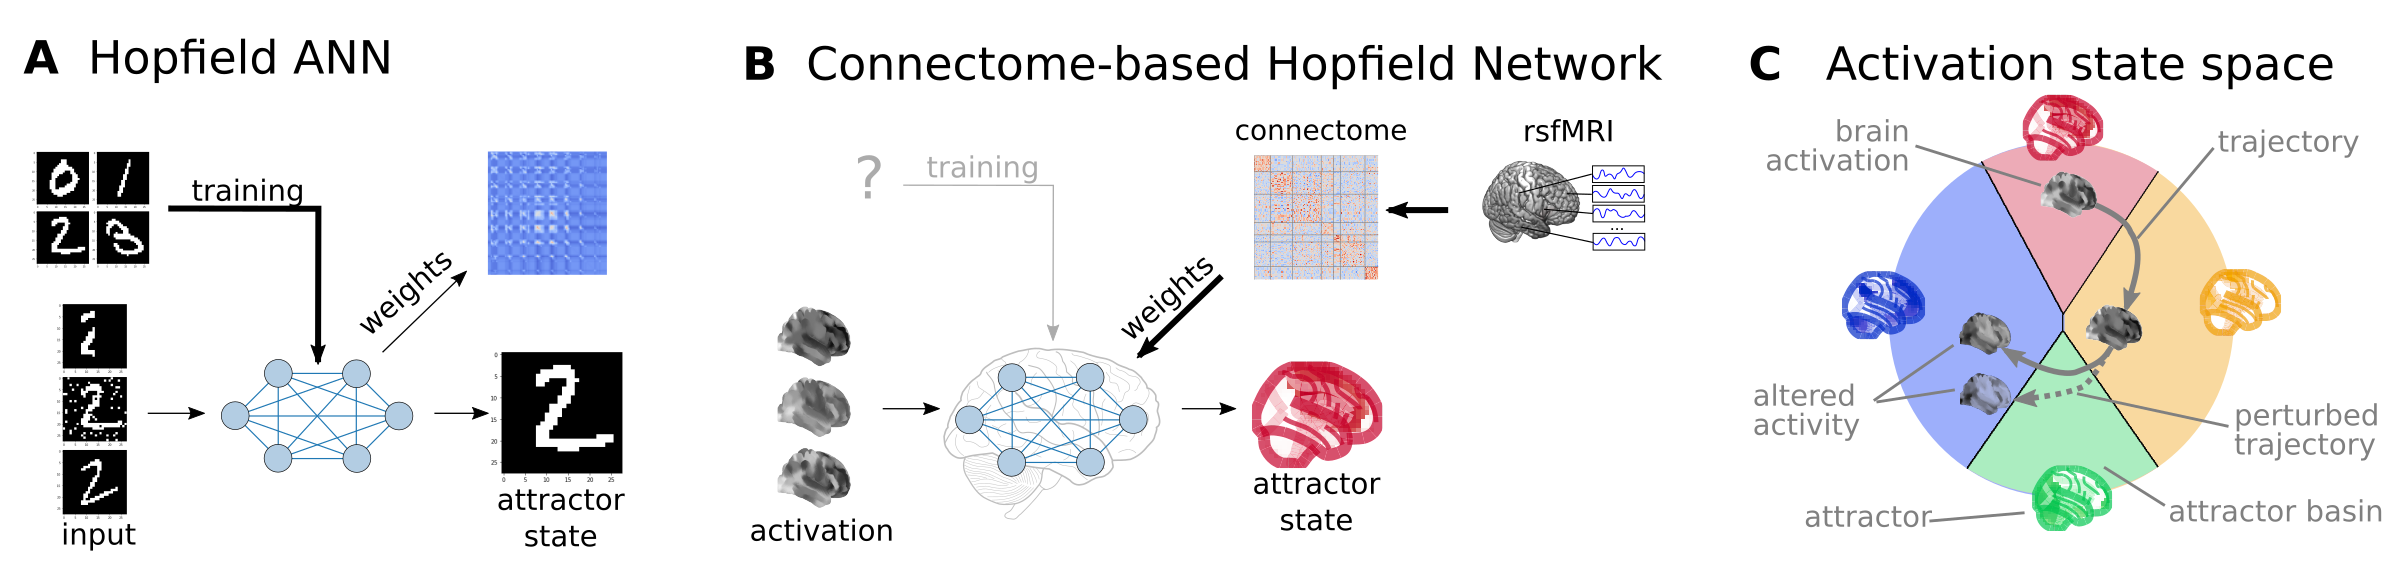
\includegraphics[width=0.7\linewidth]{files/concept-233a40c024c5a62b6a504ff1c18e4ce2.png}
\caption[]{\textbf{Connectome-based Hopfield networks as models of macro-scale brain dynamics.} \newline
\newline

\textbf{A} Hopfield artificial neural networks (HNNs)  are a form of recurrent artificial neural networks that serve as content-addressable
("associative") memory systems. Hopfield networks can be trained to store a finite number of patterns (e.g. via
Hebbian learning a.k.a. "fire together -  wire together"). During the training procedure, the weights of the HNN are trained so that the stored
patterns become stable attractor states of the network. Thus, when the trained network is presented partial, noisy or corrupted
variations of the stored patterns, it can effectively reconstruct the original pattern via an iterative relaxation
procedure that converges to the attractor states.
\textbf{B} We consider regions of the brain as nodes of a Hopfield network. Instead of training the Hopfield network to
specific tasks, we use the set its weights empirically, with the interregional activity flow estimated via functional
brain connectivity. Following form the strong analogies between the relaxation rule of Hopfield networks and the
activity flow principle that links activity to connectivity in brain networks, we propose the constructed
connectome-based Hopfield neural network (CHNN) as a computational model for macro-scale brain dynamics.\newline
\textbf{C} The proposed computational framework assigns an energy level, an attractor state and a position in a
low-dimensional embedding to brain activation patterns. Additionally, it models how the entire state-space of viable
activation patterns is restricted by the dynamics of the system and how alterations in activity and/or connectivity
modify these dynamics.}
\label{concept}
\end{figure}

In this simplistic yet powerful framework, both spontaneous and task-induced brain dynamics can be conceptualized as a
winding, high-dimensional path that meanders on the energy landscape, restricted by the "gravitational pull" of the
attractors states.
The framework provides a generative model for both resting state and task-related brain dynamics, offering novel
perspectives on the mechanistic origins of resting state brain states and task-based activation maps.

In the present work, we first explore the attractor states of the functional brain connectome and construct a
low-dimensional representation of the energy landscape.
Subsequently, we rigorously test the proposed model through a series of experiments, conducted on data obtained
from 8 experimental and clincial studies, encompassing a total of n$\approx$2000 individuals.
These analyses evaluate the robustness and replicability of the proposed approach and test its ability to reconstruct
various characteristics of resting state brain dynamics, as well as its capacity to detect and explain changes induced
by experimental tasks or alterations characteristic to brain disorders.

These experiments provide converging evidence for the validity of connectome-based Hopfield neural networks as models
of brain dynamics, and highlight their potential to provide a fresh perspective on a wide range of research questions
in basic and translational neuroscience.

\subsection{Main}\label{Main}

\subsubsection{Connectome-based Hopfield network as a model of brain dynamics}\label{Connectome-based Hopfield network as a model of brain dynamics}

First, we explored the attractor states of the functional connectome in a sample of n=41 healthy young
participants (Table~\ref{tab-samples}). We estimated interregional activity flow \citep{cole2016activity, ito2017cognitive}
as the study-level average of regularized partial correlations among the resting state fMRI timeseries of m = 122
functionally defined brain regions (BASC brain atlas, see Methods for details). We then used the standardized
functional connectome as the $w_{ij}$  weights of a continuous-state Hopfield network
\citep{hopfield1982neural, koiran1994dynamics} consisting of $m$ neural units, each having an activity
$a_i \in [ -1,1] \subset \mathbb{R})$. Hopfield networks can be initialized by an arbitrary activation pattern (consisting of
$m$ activation values) and iteratively updated (i.e. "relaxed") until convergence to one of the finite attractor states is reached. The relaxation procedure is based in a simple rule; in each iteration, the activity of a region is constructed as the weighted average of the activities of all other regions, with weights defined by the connectivity between them.
This can be expressed by the following equation:

\begin{equation}
\label{hopfield-update}
\dot{a}_i = S(\beta \sum_{j=1}^m w_{ij}a_j - b_i)
\end{equation}

where $\dot{a}_i$ is the activity of neural unit $i$ in the next iteration and $S(a_j)$ is the sigmoidal activation
function $S(a) = tanh(a)$ and $b_i$ is the bias of unit $i$ and $\beta$ is the so-called temperature parameter. For the sake of simplicity, we set $b_i=0$ in all our experiments. We refer to this architecture as a connectome-based
Hopfield neural network (CHNN). Importantly, the relaxation of a CHNN model can be conceptualized as the repeated
application of the activity flow principle \citep{cole2016activity, ito2017cognitive} , simultaneously for all
regions: $\dot{a}_i = \sum_{j=1}^m w_{ij}a_j$. The update rule also exhibits strong analogies with the inner workings
of neural mass models \citep{breakspear2017dynamic} as applied e.g. in dynamic causal modeling(see Discussion for
further details).

Hopfield networks assign an energy value to each possible activity configuration (see Methods), which decreases during
the relaxation procedure until reaching an equilibrium state with minimal energy (Figure~\ref{attractors}A, top panel,
\citep{hopfield1982neural, koiran1994dynamics}.
We used a large number of random initializations to obtain all possible attractor states of the connectome-based
Hopfield network in study 1 (Figure~\ref{attractors}A, bottom panel).

\begin{figure}[!htbp]
\centering
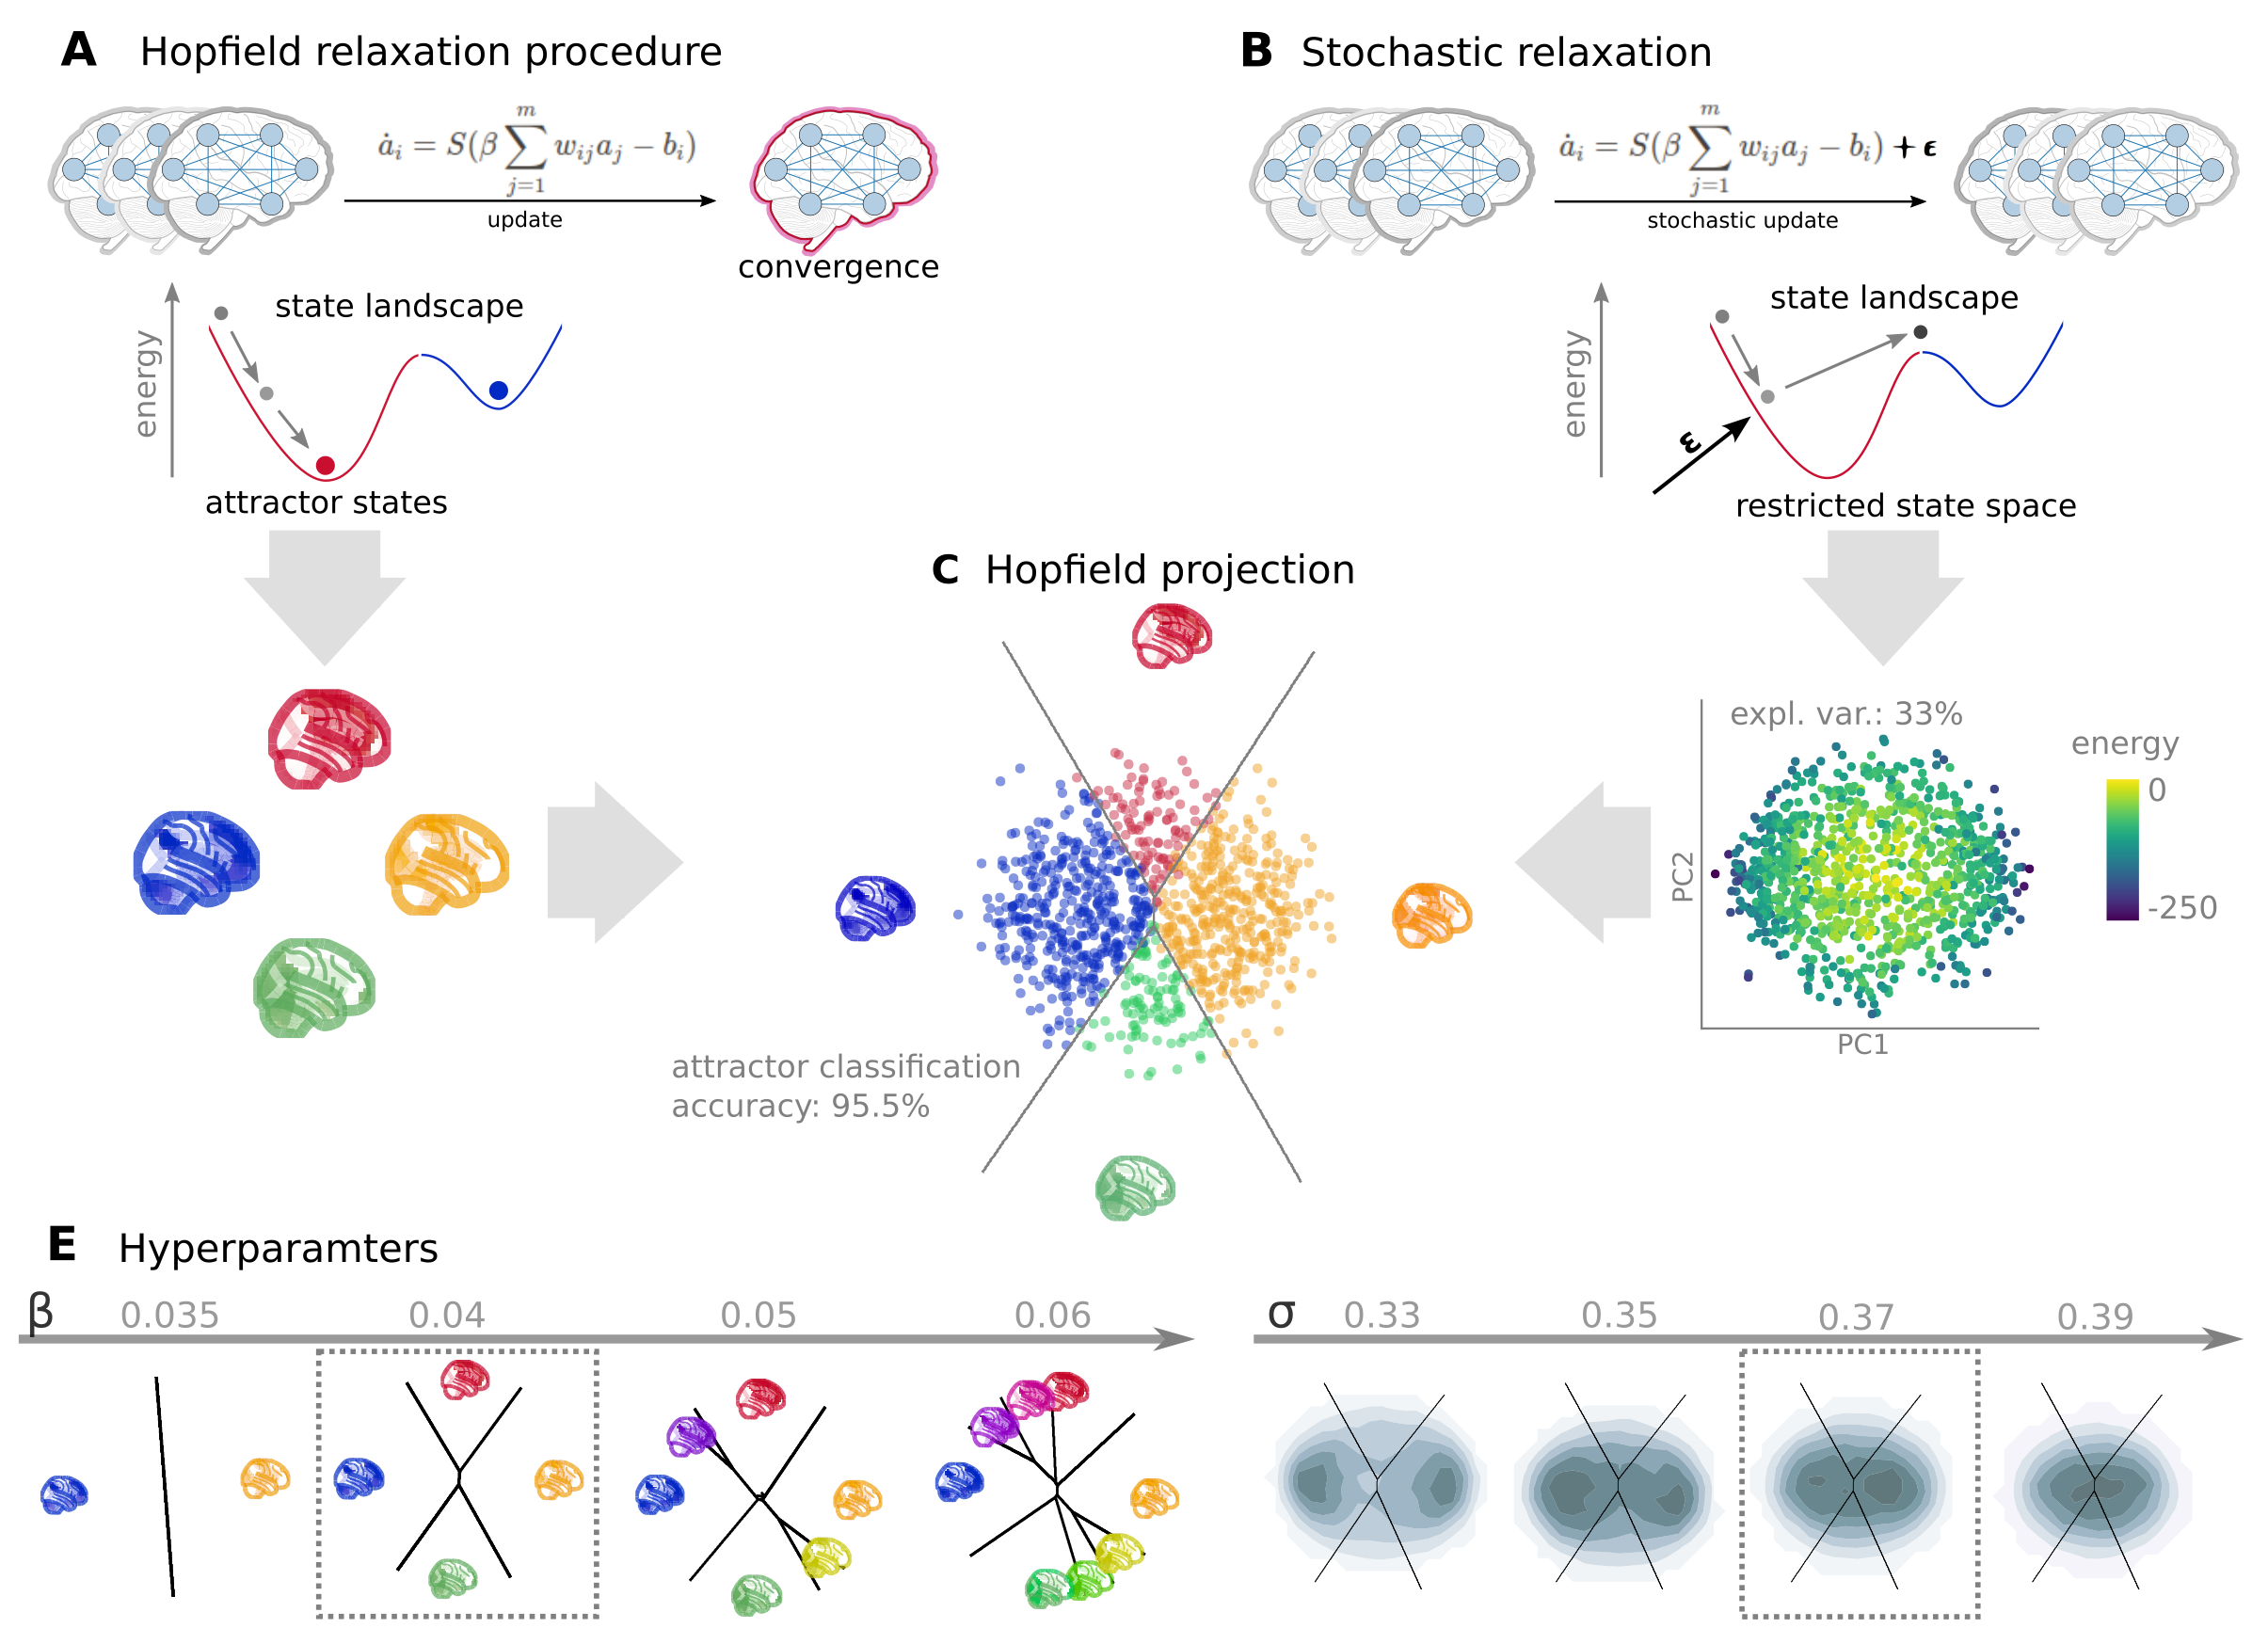
\includegraphics[width=0.7\linewidth]{files/embedding_method-d4c4bafbeada579934febaccf375be46.png}
\caption[]{\textbf{Attractor states and state-space dynamics of connectome-based Hopfield networks} \newline
\newline

\textbf{A} Top: During so-called relaxation procedure, activities in the nodes of a connectome-based Hopfield network (CHNN)
are iteratively updated based on the activity of all other regions and the connectivity between them. The energy of a
connectome-based Hopfield network decreases during the relaxation procedure until reaching an equilibrium state with
minimal energy, i.e. an attractor state. Bottom: Four attractor states of the CHNN deerived from the
group-level functional connectivity matrix from Table~\ref{tab-samples} (n=44).
\textbf{B} Top: Similarly to stochastic dynamic causal modeling, in presence of weak noise (stochastic update), the system
does not converge to an equilibrium anymore. Instead, it the system transverses on the state landscape in a way
restricted by the topology of the connectome and the "gravitational pull" of the attractor states. Bottom: We sample
the state space by running the stochastic relaxation procedure for an extended amount of time (e.g. 100.000 consecutive
stochatsic updates), each point representing a possible activation configuration (state). To construct a
low-dimensional representation of the state space, we take the first principal components of the simulated activity
patterns. The first two principal components explain approximately 55-85\% of the variance of state energy (depending
on the noise parameter $\sigma$, see Supplementary Material \textbf{X}).
\textbf{C} We map all states of the state space sample to their corresponding attractor state, with the conventional
Hopfield relaxation procedure (A). The four attractor states are also visualized in their corresponding position on the
PCA-based projection. The first two principal components yield a clear separation of the attractive state basins
(cross-validated classification accuracy: 95.5\%, Supplementary Material \textbf{X}). We refer to the resulting visualization
as the Hopfiled projection and use it to visualize CHNN-derived and empirical brain dynamics throughout the rest of
the manuscript.
\textbf{E} At its simpliest form, the CHNN framework entails only two free hyperparamters: the temperature parameter
$\beta$ (left) that controls the number of attractor states and the noise parameter of the stochastic relaxation
$\sigma$. To avoid overfitting these parameters to the empirical data, we set $\beta=0.04$ and $\sigma=0.37$ for the
rest of the paper  (dotted boxes).}
\label{attractors}
\end{figure}

Consistent with theoretical expectations, we observed that increasing the temperature parameter $\beta$ led to an
increasing number of attractor states ((Figure~\ref{attractors}E, left), appearing in symmetric pairs
(i.e. $a_i^{(1)} = -a_i^{(2)}$). For simplicity, we set the temperature parameter for the rest of the paper to a value
resulting in 4 distinct attractor states ($\beta=0.4$).

Connectome-based Hopfield networks, without any modifications, always converge to an equilibrium state.
To incorporate stochastic fluctuations in neuronal activity \citep{robinson2005multiscale}, we introduce weak
Gaussian noise to the CHNN relaxation procedure. This procedure, referred to as stochastic relaxation, prevents the
system from reaching equilibrium and, somewhat similarly to stochastic DCM \citep{daunizeau2012stochastic}, induces
complex system dynamics  (equivalent to brain activity fluctuations in our framework). Such a system may traverse extensive
regions of the state space, in a way largely shaped by the "gravitational pull" (the so-called "basins") of multiple attractor states (Figure~\ref{attractors}B).

We hypothesise that the resulting dynamics capture essential characteristics of spontaneous activity fluctuations in
the brain and can serve as a valuable generative computational model for large-scale brain dynamics. To sample the
resulting state space, we obtained 100,000 iterations of the stochastic relaxation procedure with a Hopfield network
initialized with the mean functional connectome in study 1. Next, in order to enhance interpretability, we conducted a
principal component analysis (PCA) on the resulting state space sample and obtained the first two principal components.
These components were used to construct a low-dimensional embedding (Figure~\ref{attractors}B, bottom plot).

The PCA embedding exhibited high consistency across different values of $\beta$ and $\sigma$ (Figure~\ref{attractors}E).
For all subsequent analyses, we set $\sigma=0.37$, which was determined through a coarse optimization procedure aimed
at reconstructing the bimodal distribution of empirical data in the same projection (Figure~\ref{attractors}E,
see Methods for details). On the low-dimensional embedding, which we refer to as the \textit{CHNN projection}, we observed
a clear separation of the attractor states (Figure~\ref{attractors}C), with the two symmetric pairs of attractor states
located at the extremes of the first and second PC. To map the attractor basins on the space spanned by the first two
PCs (Figure~\ref{attractors}C), we obtained the attractor state of each point visited during the stochastic relaxation
and fit a multinomial logistic regression model to predict the attractor state from the first two PCs. The resulting
accurately predicted the attractor state of arbitrary brain activity patterns,
achieving an out-of-sample accuracy of 96.5\%. The attractor basins were
visualized by using the decision boundaries obtained from this model. (Figure~\ref{attractors}C). We propose the 2-dimensional CHNN
projection depicted on (Figure~\ref{attractors}C) as a simplified representation of brain dynamics, and use it as a basis
for all subsequent analyses in this work.

\subsubsection{Reconstruction of resting state brain dynamics}\label{Reconstruction of resting state brain dynamics}

The spatial patterns of the obtained attractor states exhibit high neuroscientific relevance and closely resemble previously described large-scale brain systems. (Figure~\ref{rest-validity}A). The first pair of attractors (mapped on PC1, horizontal axis) resemble the two complementary ``macro'' systems described, among others, by \citet{golland2008data} and \citet{cioli2014differences} as well as the two "primary" brain states observed by \citet{chen2018human} and the dysphoric and anxiosomatic clusters that emerge as targets for circuit-based neuromodulation \citep{siddiqi2020distinct}. A common interpretation of this state-pair is that it consists of (i) an ``extrinsic'' system
which exhibits a stronger direct connection to the immediate sensory environment and (ii) an "intrinsic" system, whose
activity is primarily associated with dynamic changes in higher-level internal context and closely linked to the default
mode network.
The other pair of attractors spans an orthogonal axis connecting regions that are commonly associated
with perception--action cycles \citep{fuster2004upper} and recruits regions associated with active inference (e.g. motor cortices) and perceptual inference (e.g visual cortices).

\begin{figure}[!htbp]
\centering
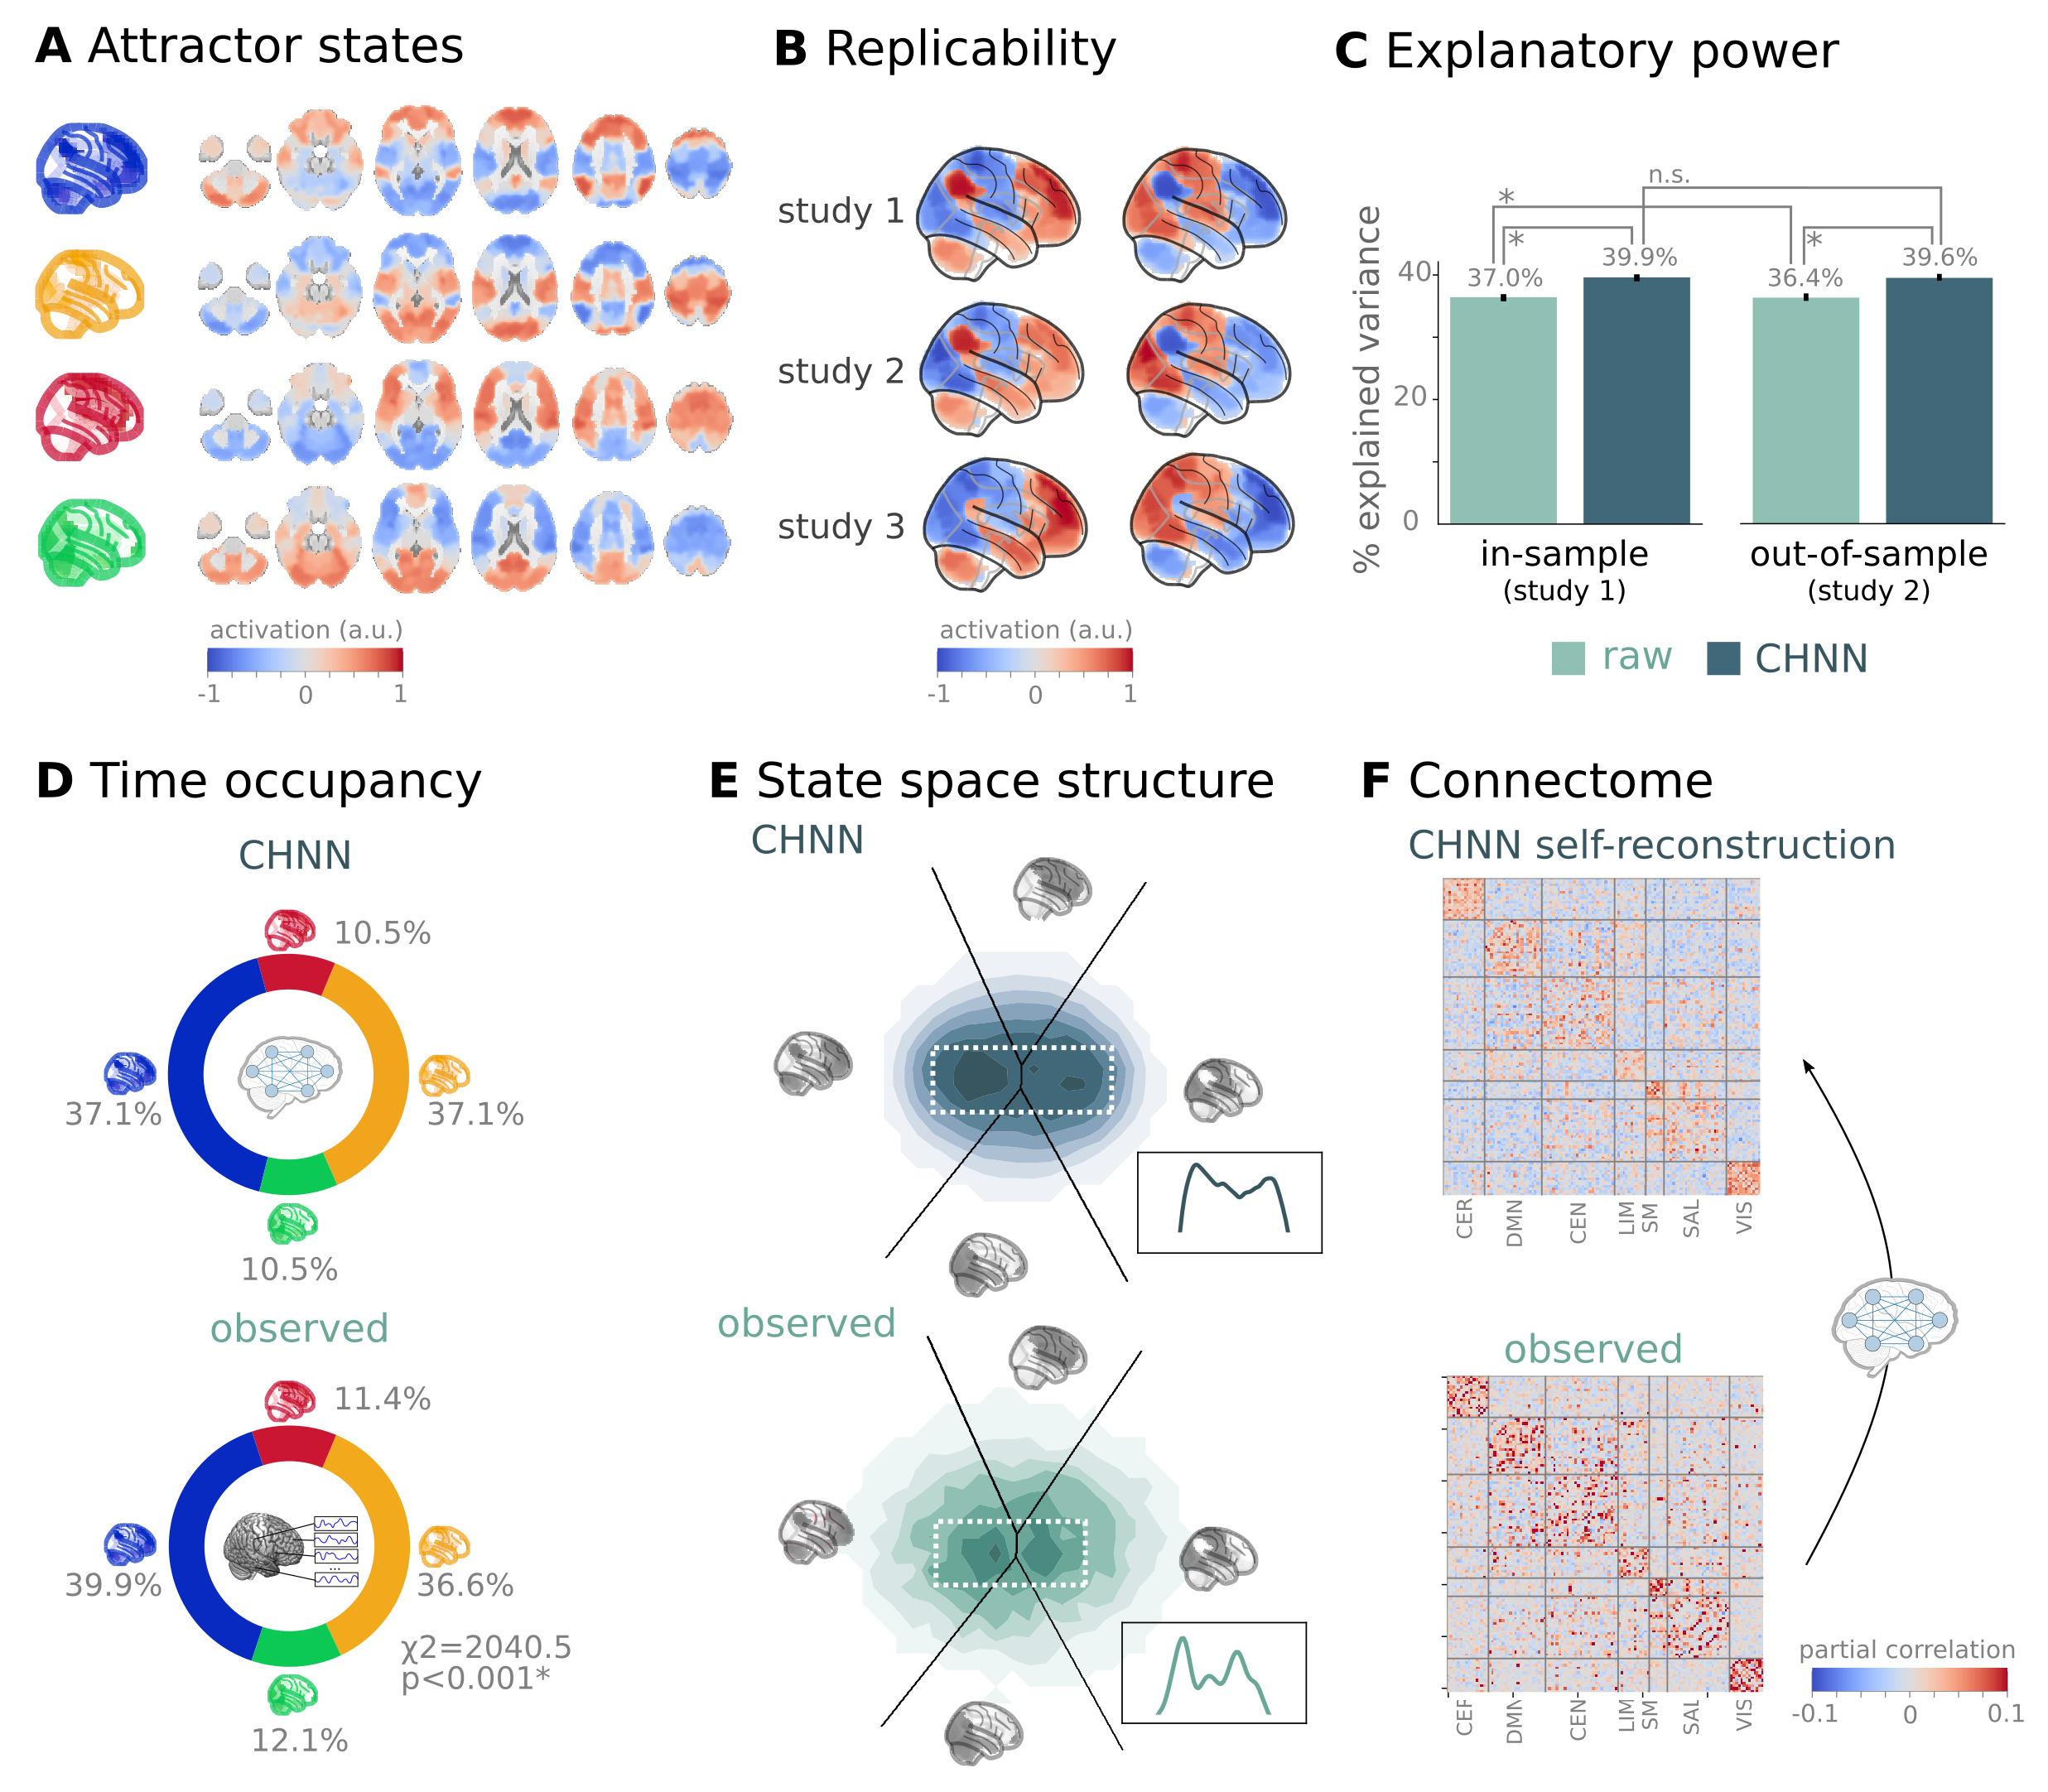
\includegraphics[width=0.7\linewidth]{files/face_validity-6e10d478356599e00a4dcef3670214d3.png}
\caption[]{\textbf{Connectome-based Hopfield networks reconstruct characteristics of real resting state brain activity.}\newline
\newline

\textbf{A} The four attractor states of the CHNN model from study 1 reflect brain activation
patterns with high neuroscientific relevance, representing sub-systems previously associated with 'internal context'
(blue), "external context" (yellow), "action/execution" (red) and "perception" (green)
\citep{golland2008data, cioli2014differences, chen2018human, fuster2004upper}.
\textbf{B} The attractor states show excellent replicability in two external datasets (study 2 and 3, mean correlation 0.93).
\textbf{C} The CHNN projection (first two PCs of the CHNN state space) explains significantly more variance (p\textless 0.0001) in the real
resting state fMRI data than principal components derived from the real resting state data itself and generalizes
better (p\textless 0.0001) to out-of-sample data (study 2). Error bars denote 99\% bootstrapped confidence intervals.
\textbf{D} The CHNN analysis accurately predicts (p\textless 0.0001) the fraction of time spent on the basis of the four attractor
states in real restring state fMRI data (study 1) and,
\textbf{E}, reconstructs the characteristic bimodal distribution of the real resting state data.
\textbf{F} Stochastic CHNNs are capable of self-reconstruction: the timeseries resulting from the stochastic relaxation procedure
mirror the co-variance structure of the functional connectome the CHNN model was initialized with.}
\label{rest-validity}
\end{figure}

Importantly, the discovered attractor states demonstrate a remarkable level of replicability (mean Pearson's
correlation 0.93) across the discovery datasets (study 1) and two independent replication datasets
(Table~\ref{tab-samples}, Figure~\ref{rest-validity}C).

Further analysis in study 1 showed that connectome-based Hopfield models accurately reconstructed multiple
characteristics of true resting-state data.

First, the CHNN projection accounted for a substantial amount of
variance in the real resting-state fMRI data in study 1 (mean $R^2=0.399$) and generalized well to out-of-sample data (study 2)
(mean $R^2=0.396$)  (Figure~\ref{rest-validity}E). Remarkably, the explained variance of the
CHNN projection significantly exceeded that of a PCA performed directly on the real resting-state fMRI data itself
($R^2=0.37$ and $0.364$ for in- and out-of-sample analyses).

Second, CHNN analyses accurately reconstruct true resting state brain state dynamics. During stochastic relaxation, the
CHNN model spends approximately three-quarters of the time on the basis of the first two attractor states, with an
equal distribution between them. The remaining one-quarter of the time is spent on the basis of the second pair of
attractor states, also equally distributed. To test whether we see similar state occupancy ratios in real resting state data,
we obtained normalized and cleaned mean timeseries in $m=122$ regions from all participants in study 1 and calculated
the attractor state of each time-frame via the CHNN model. We observed strikingly similar temporal occupancies to those
predicted by the model ($\Chi^2$-test with the null hypothesis of uniform occupancies: p\textless 0.00001,
Figure~\ref{rest-validity}B).

Third, CHNNs successfully reproduce fine-grained details of the bimodal distribution observed in the real resting-state fMRI data when projected onto the CHNN projection (Figure~\ref{rest-validity}F and Figure~\ref{attractors}E), suggesting that brain dynamics
are governed by a limited number of attractor states that emerge from the flow of activity across functional
connectivity networks.

Finally, during the stochastic relaxation procedure, CHNNs were found to generate regional time series that
preserve the covariance structure of the real functional connectome used for network initialization. This
important result indicates that a dynamic system in which activity flows across nodes of a complex network inevitably
"leaks" its underlying structure into the activity time series, providing a high level of construct validity for the
proposed approach (Figure~\ref{rest-validity}D).

It is important to reiterate that the proposed model was neither explicitly informed about, nor trained or optimized to reconstruct any of the investigated spatial (bi-modal distribution, explanatory performance) or temporal patterns (temporal state occupancy) of the brain.
The ability of the proposed connectome-based Hopfield model to reconstruct all these characteristics of real data strongly suggests that it captures essential relationships between the topology of the brain's functional connectome and the dynamics of its activation.

\subsubsection{An explanatory framework for task-based brain activity}\label{An explanatory framework for task-based brain activity}

The proposed framework offers a natural account for how activation patterns in the brain dynamically emerge form the
underlying functional connectivity. To illustrate this, we obtained task-based fMRI data from a study by
\citet{woo2015distinct} (Table~\ref{tab-samples}, n=33, see Figure~\ref{rest-validity}), investigating the neural
correlates of pain and its self-regulation. We found that time-frames obtained from periods with pain stimulation
(taking into account hemodynamics, see Methods for details) locate significantly differently on the CHNN projection
than time-frames obtained from periods without pain stimulation (permutation test, p\textless 0.001, Figure~\ref{task-validity}A,
left). Energies, as defined by the Hopfield model, were also significantly different between the two conditions
(permutation test, p\textless 0.001), with higher energies during pain stimulation.

When participants were instructed to up- or down-regulate their pain sensation (resulting in increased and decreased
pain reports and differential brain activity in the nucleus accumbens, NAc, (see \citep{woo2015distinct} for details)
we observed further changes of the location of momentary brain states on the Hopfield-projection (permutation test,
p\textless 0.001, Figure~\ref{task-validity}A, right). Interestingly, self-regulation did not manifest in significant energy changes
(permutation test, p=0.36).

\begin{figure}[!htbp]
\centering
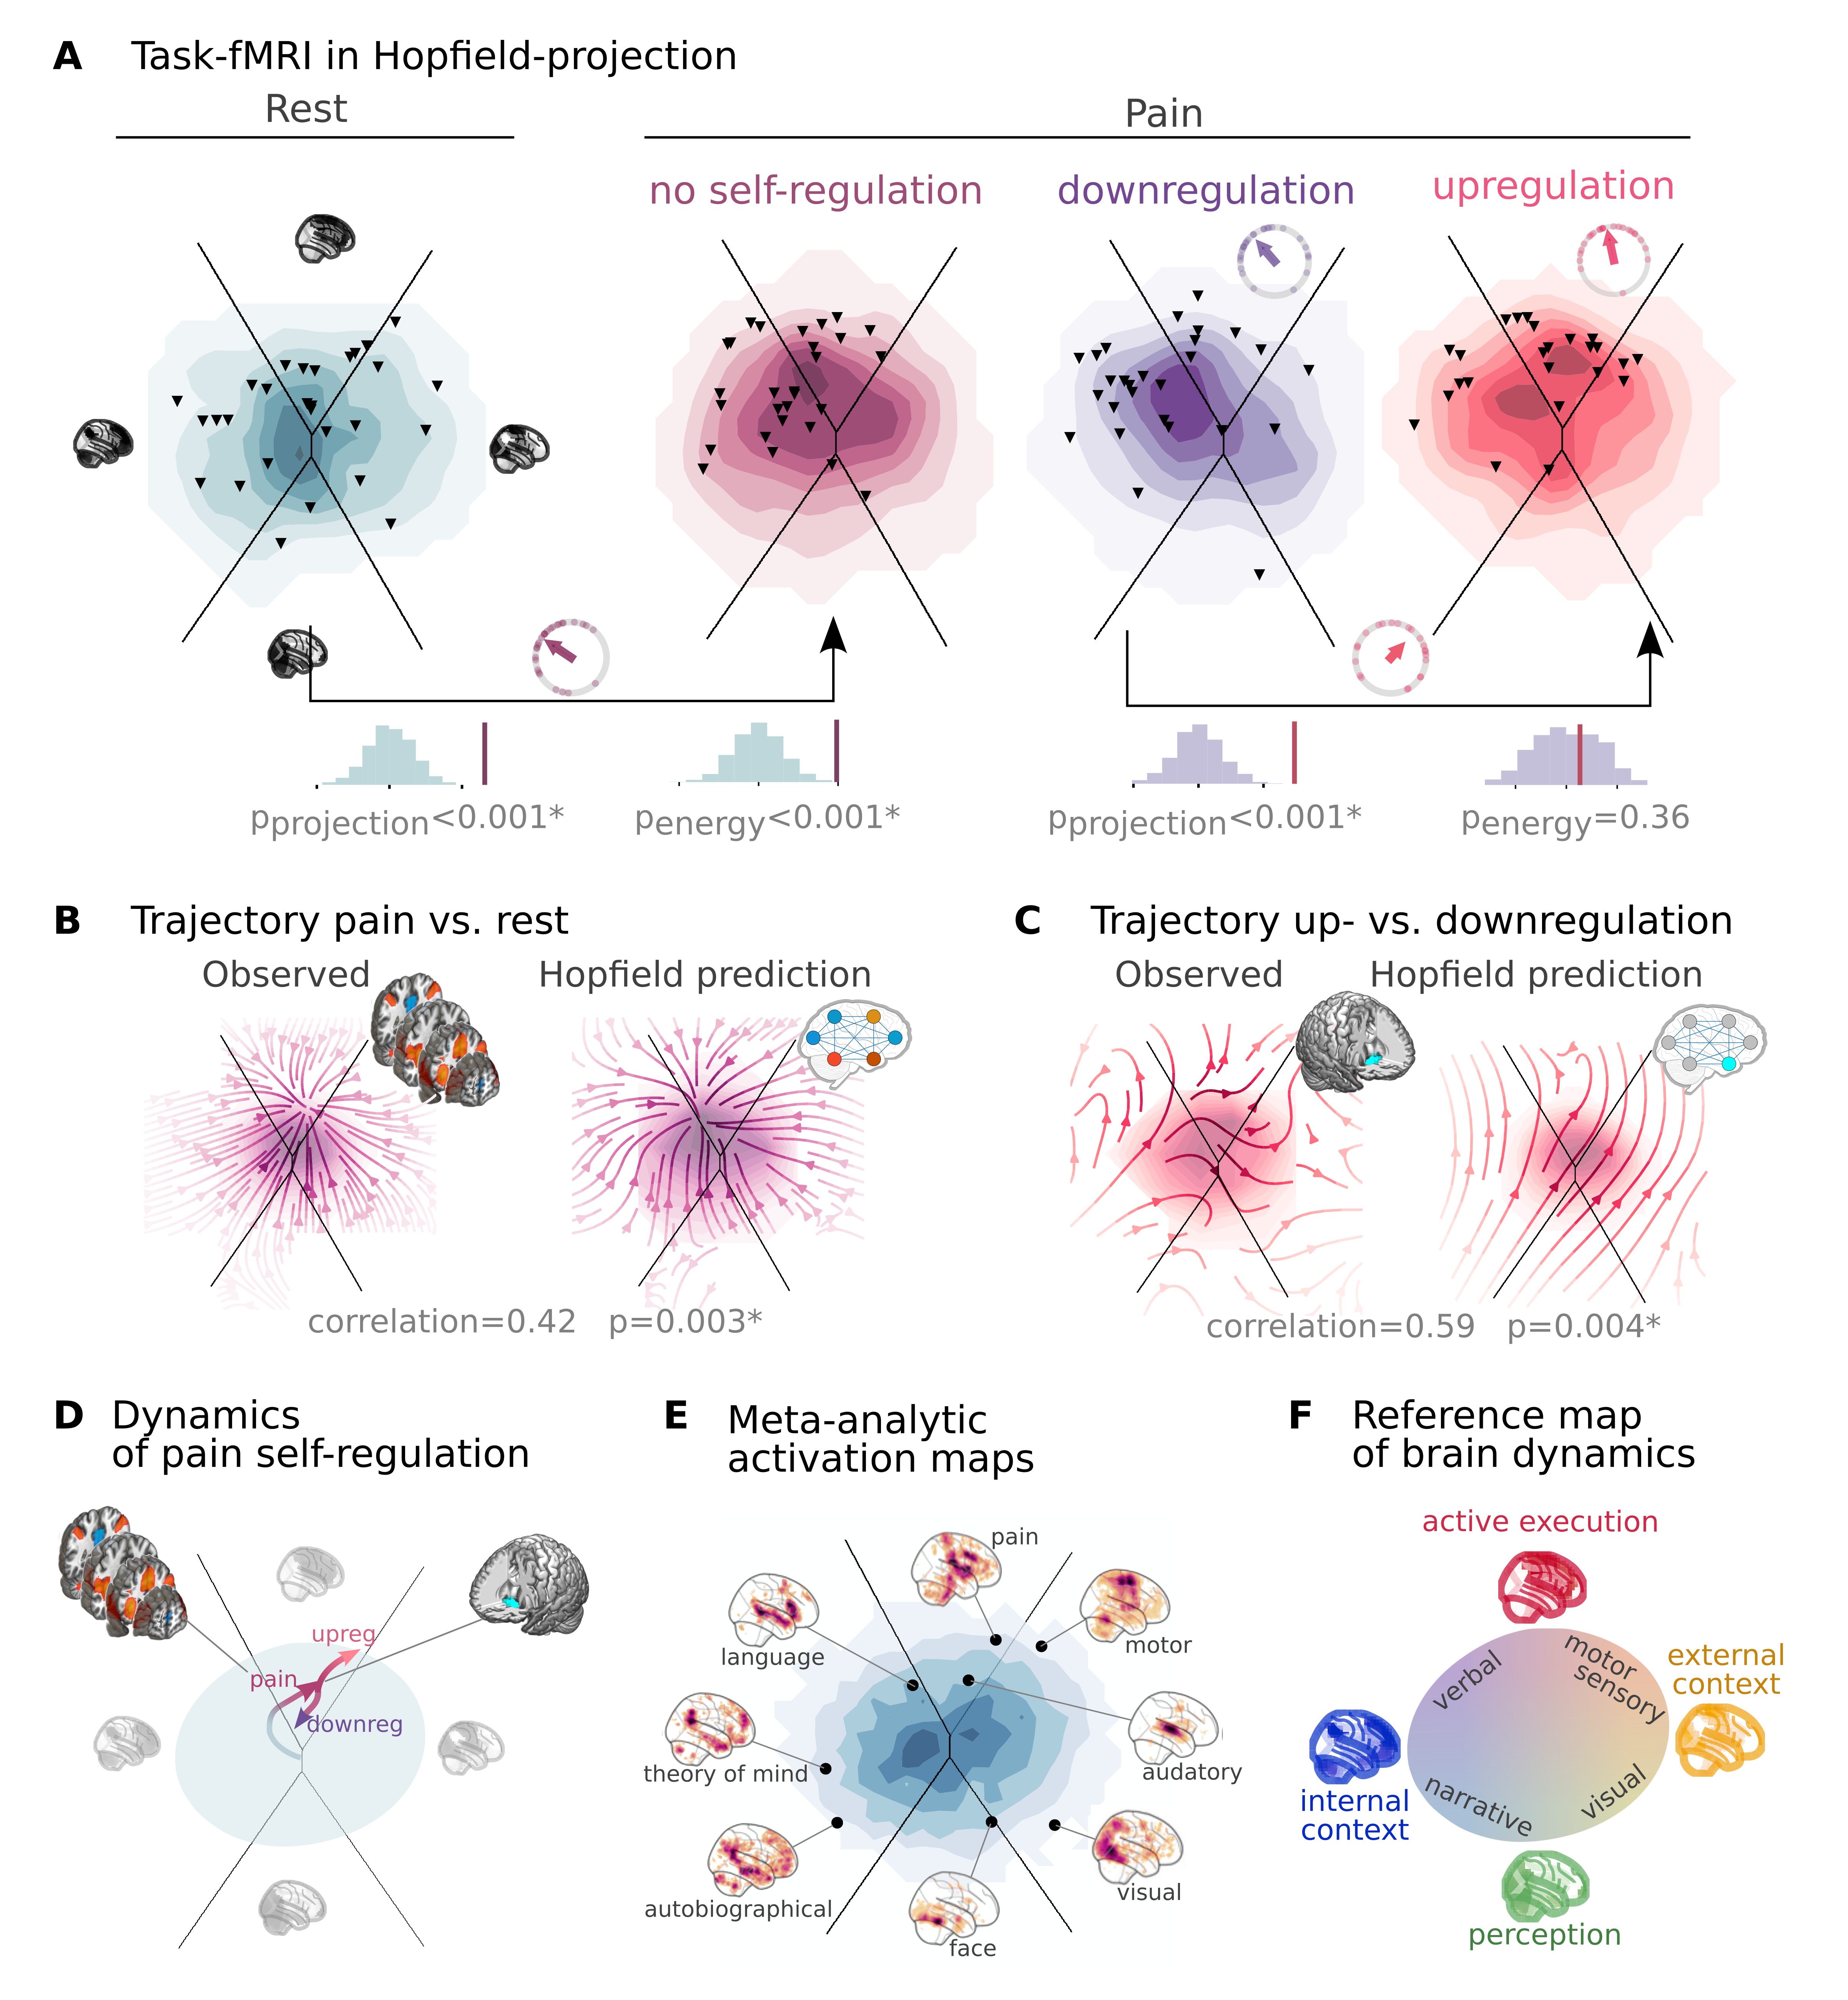
\includegraphics[width=0.7\linewidth]{files/task_validity-dd005ea46bac749a115c9f3996eabeee.png}
\caption[]{\textbf{Empirical Hopfield-networks reconstruct real task-based brain activity.} \newline

\textbf{A} Functional MRI time-frames during pain stimulation from Table~\ref{tab-samples} (second CHNN projection plot)
and self-regulation (third and fourth) locate significantly differently on the CHNN projection than brain states
during rest (first projection, permutation test, p\textless 0.001 for all).  Energies, as defined by the Hopfield model, are also
significantly different between rest and the pain conditions (permutation test, p\textless 0.001), with higher energies during
pain stimulation. Triangles denote participant-level mean activations in the various blocks (corrected for
hemodynamics). Circle plots show the directions of the change for each individual (points) as well as the mean direction
across participants (arrow), as compared to the reference state (downregulation for the last circle plot, rest for all
other circle plots).
\textbf{B} Flow-analysis of the single time-frames (based on the vector pointing to the next time-frame)
reveal a non-linear difference in brain dynamics during pain and rest (left). When introducing weak
pain-related signal in the CHNN model during stochastic relaxation, it accurately reproduces these non-linear flow
differences (right).
\textbf{C} Simulating activity in the nucleaus accumbens (NAc) (as observed by \cite{woo2015distinct}) reconstructs the observed non-linear flow difference between up- and downregulation (left).
\textbf{D} Schematic representation of brain dynamics during pain and its up- and downregulation, visualized on the CHNN
projection. In the proposed framework, pain does not simply elicit a direct response in certain regions, but instead, shifts spontaneous brain dynamics towards the "action" subsystem, converging to a characteristic "ghost
attractor" of pain. Up-regulation by NAc de-activation exerts force towards a similar direction (thus increasing the probability of the emergence of "pain-activations") while down-regulation
by NAc activation exhibit an opposite effect on brain dynamics, leading to the brain less frequent "visiting"
pain-associated states.
\textbf{E} Visualizing meta-analytic activation maps on the CHNN projection captures intimate relations between the corresponding tasks and \textbf{F} serves as a basis for a CHNN-based theoretical interpretative framework for spontaneous and task-based brain dynamics. In the proposed framework, task-based activity is not a mere response to external stimuli in certain brain locations but a perturbation of the brain's characteristic dynamic trajectories, constrained by the underlying functional connectivity. From this perspective, "activity maps" from conventional task-based fMRI analyses capture time-averaged differences in these whole brain dynamics.}
\label{task-validity}
\end{figure}

These results provide an intuitive account for how the underlying functional connectivity of the brain can give rise to
different activation patterns, depending on the current (extrinsic or intrinsic) input. In the CHNN framework, change in
input (i.e. a task or stimulation) does not simply switch to the brain into a distinct "mode" of operation but acts as
a perturbation of the system's dyanmics, resulting in mean activations changes that are only reliable measurable over
an extended period of time, as done by conventional task-based fMRI analyses.

The proposed framework offers much more than visualization and inference of resting state and task based data on the
CHNN projection. It provides a generative model for observed activity changes, enabling the prediction of brain
activity under different conditions. To illustrate this, we used the CHNN approach to simulate brain activity during pain
stimulation and self-regulation. First, we registered the frame-to-frame transitions (i.e. the vector on the 2-dimensional CHNN projection, pointing from a time-frame to the next one) in the real fMRI data for all four
conditions: rest, pain without self-regulation, downregulation, and upregulation.

Next, we evaluated the average direction in different segments of the projection plane, on a 6x6 grid. Finally, we
computed the difference between the mean directions observed during rest and pain (without regulation,
Figure~\ref{task-validity}B, left side), as well as between down- and upregulation (Figure~\ref{task-validity}C, left side).
This analysis unveiled non-linear trajectory patterns, indicating the most probable change in brain activity from a
given activity pattern, in a particular condition (pain without self-regulation or upregulation), as
compared to the reference state (rest and downregulation, respectively). In the case of pain versus rest, brain
activity tends to gravitate towards a distinct state, which we term the "ghost attractor" of pain (similar to \cite{vohryzek2020ghost}). In terms of attractor states, this belongs to the basin of the
attractor corresponding to action/execution. In case of up vs. downregulation, brain activity is pulled generally
towards a similar direction, but with a lack of a clear ghost attractor and, from most starting point, likely resulting in states that are closer to the pain-related "ghost attractor" point.

Next, our objective was to evaluate the extent to which the proposed framework can reconstruct the observed non-linear
dynamics. To simulate the alterations in brain dynamics during pain stimulation, we acquired a meta-analytic pain
activation map \citep{zunhammer2021meta} (n=603) and incorporated it as additional signal, along with Gaussian noise,
during the stochastic relaxation procedure. While incorporating such a signal naturally induces a minor linear shift
on the CHNN projection for each state generated during the stochastic relaxation procedure, this alone could not explain
the observed nonlinear dynamics in the real data (Supplementary material \textbf{X}). After conducting a
coarse-grained optimization across five different signal-to-noise (SNR) values (logarithmically spaced between
0.001 and 0.1), we found that by adding a minimal amount of signal (SNR = 0.01), the CHNN model achieved a remarkably
precise reconstruction of the observed non-linear disparities in brain dynamics between the pain and rest conditions,
including the characteristic pain-related "ghost attractor". (Spearman's $\rho$ = 0.42, p=0.003,
Figure~\ref{task-validity}B, right side).

The same model was also able to reconstruct the observed non-linear differences in brain dynamics between the up- and
downregulation conditions (Spearman's $\rho$ = 0.59, p=0.004) without any further optimization (SNR=0.01,
Figure~\ref{task-validity}C, right side). The only change we made to the model was the addition (downregulation) or
subtraction (upregulation) of activation in the NAc (the region in which \citep{woo2015distinct} observed significant
changes between up- and downregulation), with an SNR of 0.01.

These findings offer novel insights into the neural mechanisms underlying pain and its self-regulation, providing a
mechanistic explanation for the involvement of both nociception-related regions and the NAc (nucleus accumbens) in pain
regulation. (Figure~\ref{task-validity}D). Additionally, these findings emphasize that the conceptual differentiation
between resting and task states may, to a considerable extent, be an artificial dichotomy. Instead, the brain remains
in a continuous state of flux, which is not radically altered by task states, even in the presence of highly salient
stimuli such as pain.

% -> discussion

To provide a comprehensive picture on how other tasks map onto the CHNN projection, we obtained various task-based
meta-analytic activation maps from Neurosynth (see Supplementary material X for details) and plotted them on the
CHNN projection (Figure~\ref{task-validity}E). This analysis demonstrated that the CHNN projection can effectively
visualize and quantify the dynamics of various cognitive processes, encompassing sensory, motor, cognitive, and social
domains. Furthermore, the analysis revealed that the two primary axes of the projection correspond well to the
differentiation between internal and external context, as well as the perception-action axis, respectively.

In this coordinate system, visual processing is labeled "external-perception", sensory-motor processes
"external-active", language, verbal cognition and working memory is labelled "internal-active" and long-term memory
as well as social and autobiographic narrative fall into the "internal-perception" regime (Figure~\ref{task-validity}F).

Our results highlight a very powerful feature of the proposed generative framework, namely that it can be used to
simulate and predict brain dynamics under different conditions. Predicting the effect of lower or higher level of
activity in certain regions (or lower or higher connectivity between them) on global brain dynamics and responses to
various tasks provides unprecedented opportunities for forecasting the effect of interventions, such as pharmacological
or non-invasive brain stimulation, on brain function.

\subsubsection{Clinical relevance}\label{Clinical relevance}

Computational models, such as the CHNN approach, have the potential to make a significant contribution to our mechanistic comprehension of various neurological and psychiatric disorders. This represents a crucial stride towards developing effective treatments. While providing a demonstration of the CHNN approach to yield such mechanistic insights in clinical populations is well outside the scope of the current study, here we present evidence that CHNN-based attractor state analysis can effectively capture and quantify several disease-related alterations in resting state brain dynamics.

For the sake of simplicity, we utilized one of the basic CHNN-based analysis methods. Specifically, we applied the CHNN model from study 1 to allocate each time-frame of resting state data to one of the 4 attractor states. Then, we compared the average activity during resting state within each state across different clinical groups (with Bonferroni correction applied across brain regions and attractor states), resulting in a total of 122*4 comparisons per dataset. We analyzed three large public clinical databases as provided by the Autism Brain Imaging Data Exchange
(Table~\ref{tab-samples}: ABIDE, \citep{di2014autism}, the Centers of Biomedical Research Excellence
(Table~\ref{tab-samples}: COBRE, \citep{aine2017multimodal}) and the Alzheimer's Disease Neuroimaging Initiative
(Table~\ref{tab-samples}: ADNI, \citep{petersen2010alzheimer}).
In these analyses, resting state fMRI data of patients with autism spectrum disorder (ASD), schizophrenia (SCZ) and Alzheimer's disease
(AD) was contrasted to their respective control groups (typically developing controls for ASD, healthy control
participants for SCH and individuals with mild cognitive impairment (MCI) for AD, respectively).

\begin{figure}[!htbp]
\centering

\includegraphics[width=0.7\linewidth]{files/state_analysis-99cf9bea7b6eb9831250ef9f99e097cd.svg}
\caption[]{\textbf{Connectome-based Hopfield analysis as a sensitive tool for the study of clinical disorders.} \newline

We quantified attractor state activations in three clinical datasets (Table~\ref{tab-samples}) as the
individual-level mean activation of all time-frames belonging to the same attractor state. CHNN analyses of attractor
state activations revealed significant differences in all three datasets.
\textbf{A} Attractor state analysis of individuals with autism spectrum disorder (ASD) and typically developing controls (TD)
captures alterations similar to those previously associated to ASD-related perceptual atypicalities as well as atypical integration of information about the ``self'' and the ``other''.
\textbf{B} The most prominent Schizophrenia (SCZ)-related differences (as compared to healthy controls (HC) are related increased
activity of the internal subsystem and increased visual activations on the basis of the attractor state associated with perception.
\textbf{C} In Alzheimer's disease (AD), CHNN analysis revealed, among others, hyperactivity in the hippocampal formation (collateral sulcus) during perception, a commonly reported finding in AD.
and internal context (both of which together host long-term memory processes, see Figure~\ref{task-validity}F). All
results are corrected for multiple comparisons across brain regions and attractor states (122*4 comparisons)
with Bonferroni-correction. See Table \textbf{X} for detailed results.}
\label{clinical-validity}
\end{figure}

We found several significant differences in the mean attractor activation of patients as compared to the respective
controls.

ASD (Figure~\ref{clinical-validity} left side) was found to be characterized by increased activity of the sensory-motor and middle cingular cortices during "action-execution" related states and increased visual and decreased sensory and auditory activity during "perception" states, likely reflecting the widely acknowledged, yet poorly understood, perceptual atypicalities in ASD \citep{hadad2019perception}.
ASD related changes in the internal-external axis were characterized by more involvement of the posterior cingulate, the precuneus, the nucleus accumbens, the dorsolateral prefrontal cortex (dlPFC), the cerebellum (Crus II and lobule VII) and inferior temporal regions during activity of the internalizing subsystem (Table \textbf{X}). While similar, default mode network (DMN)-related changes have often been attributed to an atypical integration of information about the ``self'' and the ``other'', a more detailed CHNN-analysis may help to further disentangle the specific nature of these changes.

In SCZ, the most prominent differences were found on the internal-external axis, with elevated activity in several brain regions during brain activity on the basin of the internal subsystem and decreased activity in the external subsystem. (Figure~\ref{clinical-validity}B, Table \textbf{X}). These findings are in line with the notion that, in schizophrenia, the forward projections have decreased functional connectivity relative to the back projections, and this may reduce the effects of external bottom-up inputs from the world relative to internal top-down thought processes \citep{rolls2021attractor}.
On the axis of the perception-action subsystems, the main difference was found in the visual and sensorimotor cortices, concordant with the widespread notion of visual and sensory deficits in SCZ \citep{javitt2009sensory, butler2008visual, adamek2022early}.

In the AD vs. MCI comparison, we found decreased resting state activations in several regions, including the inferior parietal lobule (IPL) and primary visual cortex, likely a consequence of high levels of amyloid-$\beta$ reducing synaptic excitatory transmission, resulting in synaptic failure and neuronal hypoactivity \citep{selkoe2002alzheimer}. A significant hyperactivity was found in the hippocampal formation (collateral sulcus) during perception states, which is
a commonly reported finding in AD \citep{aizenstein2015hippocampal, ewers2011neuroimaging}
(Figure~\ref{clinical-validity}C, \textbf{table}). Moreover, we found increased activity in supplementary motor cortex (SMA), an area that is known to display relatively little atrophy and hypomethabolism with AD and has previously brought into relation with the presevation of musical memories in AD \citep{jacobsen2015musical}.

\begin{tabular}{p{\dimexpr 0.250\linewidth-2\tabcolsep}p{\dimexpr 0.250\linewidth-2\tabcolsep}p{\dimexpr 0.250\linewidth-2\tabcolsep}p{\dimexpr 0.250\linewidth-2\tabcolsep}}
\toprule
region & state & effect size & p value \\
\hline
\newline
\textbf{Autism spectrum disorder (ABIDE)} &  &  &  \\
HESCHLS GYRUS & 1 & -0.126 & \textless 0.0001 \\
POSTERIOR\_CINGULATE\_CORTEX & 0 & 0.109 & \textless 0.0001 \\
CEREBELLUM\_VIIb\_medial & 3 & 0.104 & \textless 0.0001 \\
SOMATOMOTOR\_NETWORK\_mediolateral & 1 & -0.099 & 0.00976 \\
INFERIOR\_MARGINAL\_SULCUS & 0 & 0.098 & \textless 0.0001 \\
SUPERIOR\_TEMPORAL\_GYRUS\_middle & 1 & -0.098 & \textless 0.0001 \\
FRONTAL\_EYE\_FIELD & 1 & -0.095 & \textless 0.0001 \\
left\_SOMATOMOTOR\_NETWORK\_dorsolateral & 1 & -0.094 & 0.00976 \\
CINGULATE\_SULCUS\_posterior & 0 & 0.092 & \textless 0.0001 \\
left\_MIDDLE\_FRONTAL\_GYRUS\_posterocaudal & 2 & -0.092 & \textless 0.0001 \\
INFERIOR\_TEMPORAL\_GYRUS & 3 & 0.091 & \textless 0.0001 \\
\newline
 \textbf{Schizophrenia (COBRE)} &  &  &  \\
left\_ANGULAR\_GYRUS & 1 & -0.139 & \textless 0.0001 \\
MEDIODORSAL\_VISUAL\_NETWORK\_posterior & 1 & 0.138 & \textless 0.0001 \\
SUPERIOR\_PARIETAL\_LOBULE & 0 & 0.128 & \textless 0.0001 \\
MEDIODORSAL\_VISUAL\_NETWORK\_posterior & 0 & -0.119 & \textless 0.0001 \\
POSTERIOR\_VISUAL\_NETWORK\_dorsomedial & 1 & 0.114 & 0.00976 \\
right\_MIDDLE\_FRONTAL\_GYRUS\_anterior & 2 & -0.105 & \textless 0.0001 \\
MEDIAL\_ORBITAL\_GYRUS & 2 & -0.102 & \textless 0.0001 \\
POSTERIOR\_CINGULATE\_CORTEX & 3 & 0.102 & \textless 0.0001 \\
right\_MIDDLE\_FRONTAL\_GYRUS\_anterior & 3 & 0.101 & \textless 0.0001 \\
MEDIAL\_ORBITAL\_GYRUS & 3 & 0.099 & \textless 0.0001 \\
right\_MIDDLE\_FRONTAL\_GYRUS\_posterior & 2 & -0.098 & \textless 0.0001 \\
\newline
 \textbf{Alzheimer's disease (ADNI)} &  &  &  \\
CEREBELLUM\_IX\_middle & 0 & -0.154 & 0.00976 \\
COLLATERAL\_SULCUS & 1 & 0.139 & \textless 0.0001 \\
CEREBELLUM\_IX\_dorsal & 1 & 0.132 & 0.02928 \\
MEDIAL\_VISUAL\_NETWORK\_posterior & 0 & -0.129 & \textless 0.0001 \\
PARIETO\_OCCIPITAL\_SULCUS\_ventral & 0 & -0.128 & 0.00976 \\
PARIETO\_OCCIPITAL\_SULCUS\_ventral & 1 & 0.127 & 0.00976 \\
VENTRAL\_VISUAL\_NETWORK\_medial & 0 & -0.124 & 0.02928 \\
left\_INFERIOR\_PARIETAL\_LOBULE & 2 & -0.11 & \textless 0.0001 \\
right\_INFERIOR\_PARIETAL\_LOBULE & 2 & -0.095 & \textless 0.0001 \\
left\_CEREBELLUM\_CRUSII\_posterior & 2 & -0.094 & \textless 0.0001 \\
SOMATOMOTOR\_NETWORK\_anteromedial & 2 & 0.093 & \textless 0.0001 \\
\bottomrule
\end{tabular}

\subsection{Discussion}\label{Discussion}

Regions of the brain are in a constant flux of information exchange, giving rise to characteristic co-activations patterns.
The degree to which activation in a region triggers activation in another is different for every pair of regions, spanning an
intricate network, commonly referred to as the functional connectome.

In this study, we have introduced a simple yet robust framework that elucidates how activity propagation within the functional connectome orchestrates large-scale brain dynamics, leading to distinct brain states accompanied by characteristic dynamic responses to perturbations.
Through a series of experiments, we have demonstrated that the proposed model can effectively reconstruct and predict large-scale brain dynamics across diverse conditions.

The presented approach offers a fresh perspective on large scale brain dynamics and offers unparalleled prospects for forecasting the impact of interventions, including pharmacological treatments or non-invasive brain stimulation, on brain function.

The construct validity of our model is rooted in the activity flow principle, first introduced by
\citet{cole2016activity}. The activity flow principle states that activity in a brain region can be predicted by a weighted combination of the activity of all other regions, where the weights are set to the functional connectivity of those regions to the held-out region. This principle has been shown to hold across a wide range of experimental and clinical conditions
\citep{cole2016activity, ito2017cognitive, mill2022network, hearne2021activity, chen2018human}.

\begin{quote}
ToDo: latent FC-based modelling: \cite{McCormick_2022}
\end{quote}

Our model was born from the intuition that the repeated, iterative application of the activity flow equation in a system that exhibits close analogies with a type of recurrent artificial neural network known as Hopfield networks
\citep{hopfield1982neural}.

Hopfield networks have previously been shown to exhibit a series of characteristics that are also highly relevant for
brain function, including the ability to store and recall memories \citep{hopfield1982neural}, self-repair \citep{murre2003selfreparing},
a staggering robustness to noisy or corrupted inputs \citep{hertz1991introduction} and the ability to produce
multistable dynamics organized by the "gravitational pull" of a finite number of attractor states
\citep{khona2022attractor}. While many of such properties of Hopfiled networks have previously been proposed as a model for micro-scale neural systems (see \cite{khona2022attractor} for a review), the proposed link between macro-scale activity propagation and Hopfield networks allows transferring the vast body of knowledge on Hopfield networks to the study of large-scale brain dynamics.

Integrating Cole's activity flow principle with the Hopfield neural network architecture mandates the initiation of network weights with functional connectivity values, specifically partial correlations as suggested by \citet{cole2016activity}.
Considering the functional connectome as weights of an already trained neural network distinguishes our methodology not only from conventional computational modeling strategies, which usually rely on the structural connectome as a proxy for polysynaptic connectivity \citep{cabral2017functional}, but also from "neuroconnectomist" approaches that employ explicit training procedures \citep{doerig2023neuroconnectionist}.
Functional connectome-based Hopfield neural network (CHNN) models can be conceptualized as a streamlined alternative to those methodologies, offering significant advantages.

Firstly, the intricate nature of conventional computational models of the brain leads to an exponential proliferation of the parameter space.
While finely detailed computational models hold promise for providing comprehensive insights, they are prone to overfitting real data \citep{breakspear2017dynamic}.
In contrast to those approaches, the basic form of the CHNN approach comprises solely two hyperparameters (temperature and noise) and yields notably consistent outcomes across an extensive range of these parameter. To underscore the potency of this simplicity and stability, in the present work, we intentionally minimized the fine-tuning of these parameters. We fixed the temperature parameter at a value that robustly provides 4 attractor
states and used a single noise level for all experiments (selected with a coarse optimization procedure to approximately
mimic the distribution of real data).

Secondly, high model complexity usually translates to a greater challenge in terms of interpretability.
The CHNN approach offers straightforward interpretations, as it establishes a
direct link between two highly prevalent metrics of brain function: functional connectivity and brain activity.
This connection is not solely conceptual, but also mathematical, facilitating the exploration and prediction of alterations in the system's dynamics in response to perturbations affecting both activity and connectivity.

Given its simplicity, it is remarkable, if not surprising, how accurately the CHNN model is able to
reconstruct and predict brain dynamics under a wide range of conditions. Particularly surprising is the result
that the 2-dimensional CHNN projection can explain more variance in real resting state fMRI data than the first two principal components derived from the data itself.
Here we propose that the explanation for the extraordinary performance of the CHNN model in reconstructing brain function is that it captures essential principles of the underlying dynamics that can be used to reconstruct the brain's activation state-space even if our empirical measurements are corrupted by noise and low sampling rate.

The known noise-tolerance of the proposed architecture may also explain the high replicability of CHNN attractors across different
datasets (study 2 and 3). The observed level of replicability allowed us to re-use the CHNN model constructed with the
connectome of study 1 for all subsequent studies (2-8), without any further fine-tuning or study-specific parameter
optimization of the CHNN model.

Attractor states are a key concept in the CHNN framework. They are not only local minima in the state-space but act as a driving force for the dynamic trajectories of brain activity. Nevertheless, attractor states should not be confused with the conventional notion of brain states (e.g. co-activation patterns \citep{chen2015introducing}). In the CHNN framework, attractor states can rather be conceptualized as "Platonic idealizations" of brain activity, that are continuously approximated - but never reached - by the brain, resulting in a complex, clustered distribution of actual brain activation patterns. In or notion, this clusteredness is what gives rise to the commonly described reoccurring quasi-periodic patterns, commonly referred to as brain states.

Relying on previous work, we can establish a relatively straightforward (yet somewhat speculative) mapping between attractor states and brain function. We refer to the first two attractor states as the internal and external subsystems \citep{golland2008data, cioli2014differences}. Both CHNN-reconstructed and empirical brain activity spans the highest variance along the axis corresponding to this attractor state pair, suggesting that the robust and widely described observation of the brain state we commonly refer to as the DMN is a consequence of the brain's tendency to commute between the two state-space clusters emerging along this primary axis.
The third and fourth attractor states accurately map to the previously described perception-execution axis within the brain \citep{fuster2004upper}. The four investigated attractor states display an appealing correspondence to recent theories of brain function that capitalize on Friston's free energy principle \citep{friston2006free} and postulate the necessary existence of subsystems for active and perceptual inference \citep{friston2023free} as well as a hierarchically organized (i.e. external and internal) subsystems that give rise to consciousness \citep{ramstead2023inner}.

In the CHNN framework, the brain is in a constant state of flux, traversing extended areas of the state space. Task-based brain activity in this framework is not a mere response to external stimuli in certain brain locations but a perturbation of the brain's charcteristic dynamic trajectories, shifting towards the realms of those attractor states that represent the type of function required by the task or stimuli. In other words brain activity is only perturbed by external inpout, rather than predestined. We exemplified this with the case of the self-regulation of pain (study 4).
In our analyses, the CHNN approach was not only able to capture participant-level activity changes induced by pain and its self-regulation (showing significant differences on the CHNN projection and in terms of state energy), but also accurately predicted the non-linear changes in activity flow induced by characteristic activity changes and give a mechanistic account for how activity change in a single region (NAcc) may result in a significantly altered pain experience.

Brain dynamics can not only be perturbed by task or other types of experimental or naturalistic interventions, but also
by pathological alterations. In our analysis of clinical samples (studies 6-8), we found that CHNN-based analysis of mean attractor activations is a highly sensitive tool to characterise neural correlates of autism spectrum disorder (ASD), Schizophrenia (SCH) and Alzheimer's disease (AD), even with the most conservative correction for multiple comparisons. These results - altough descriptiuve in their nature - provide a proof-of-concept regarding the clinical potential of the proposed approach and pave the way for more elaborate applications of the CHNN approach in clinical and translational research.

Together, our findings open up a series of exciting opportunities for the mechanistic understanding of brain function.

First, the 2-dimensional CHNN projection offers a common framework for the interpretations of any brain activity patterns, and conceptualize changes related to various behavioral or clinical states or traits as a shift in brain dynamics along the axes determined by the attractor states.

Second, the CHNN model's utility extends far beyind the sole detection of such altered brain dynamics. By its generative nature, CHNN analyses may provide insights into the causes of changes in brain dynamics, by for instance, identifying the regions or connections that act as an Achilles heel in generating such changes. Such analyses could, for instance, aid the differentiation of primary causes and secondary effects of particular activity or connectivity changes in various clinical conditions.

Third, the CHNN approach might provide testable predictions about the effects of interventions on brain functions,
like pharmacological or non-invasive brain stimulation (e.g. transcranial magnetic or direct current stimulation,
focused ultrasound) or neurofeedback. Obtaining such predictions on the individual level (e.g. based on the individual functional connectome) might aid the design of personalized medicine approaches.

In this initial work, we presneted the similiest possible implementation of the CHNN concept. It is clear that the presented analyses   exploit only a small proportion of the richness of the full state-space dynamics reconstructed by the CHNN model.
There are many potential way to further improve the utility of the CHNN apporach. Increasing the number of reconstructed attractor states (by increasing the temperature parameter), investigating higher-dimensional dynamics, fine-tuned hyperparameters, the effect of
different initializations and perturbations are all important direction for future work, with the potential to further
improve the model's accuracy and usefulness.

\begin{quote}
\textbf{other potential topics}:

\begin{itemize}
\item why no HRF modelling (could be a possible extension, but it is also not part of the activity flow approach and we don't recosntruct time series, but rather activations)
\item is the connectome stationary? See arguments by the Cole-group.
\item why rs-fMRI connectome (could be latent-FC a'la McCormick, 2022)
\item the CHNN model is not a model of brain function, but a model of brain dynamics. It does not strice to explain various brain regions ability to perform certain computations, but the brain's characteristic trajectories, which are perturbed by tasks and other types of interventions.
\end{itemize}
\end{quote}

\subsection{Conclusion}\label{Conclusion}

To conclude, here we have proposed a lightweight, high-level computational framework that accurately captures and predicts brain dynamics
under a wide range of conditions. The framework models large-scale activity flow in the brain with a recurrent
artificial neural network architecture that, instead of being trained to solve specific tasks or mimic certain dynamics,
is simply initialized with the empirical functional connectome. The framework identifies neurobiologically meaningful
attractor states and provides a model for how these restrict brain dynamics. The proposed framework, referred to as the
connectome-based Hopfield neural network (CHNN) model, can accurately reconstruct and predict brain dynamics under a wide range of
conditions, including resting state, task-induced activity changes, as well as in various brain disorders. CHNNs establish a conceptual link between connectivity and activity provide and offer a simple, robust, and highly interpretable computational alternative to the conventional descriptive approaches to investigating brain function. The generative nature of the proposed model opens up a series of exciting opportunities for future research, including novel ways of assessing causality and mechanistic understanding, and the possibility to predict the effects of various interventions, thereby paving the way for novel personalized medical approaches.

\subsection{Methods}\label{Methods}

\subsubsection{Hopfield network}\label{Hopfield network}

We employ an empirical, connectome-based Hopfield neural network (CHNN) as a means to model brain activation and dynamics, aiming to
bridge the gap between classical computational modeling and neuroconnectionism. The architecture of the Hopfield network
\citep{hopfield1982neural} consists of a single layer of fully connected nodes, the undirected weights connecting
all the nodes serve as the system's memory.
Instead of training the weights on known patterns, we initialize the weights with a group-level
connectivity matrix; each node in the network representing a brain region. Through its associative memory capabilities,
the network can retrieve patterns embedded within its memory, when presented with an input similar to a target
pattern. During the retrieval process, the network will iterate on the output pattern until the system converges to a
stable state, a so-called attractor state. The mathematical energy of all possible states of a trained Hopfield network
spans an N dimensional, multi-stable state landscape. This landscape constrains the state configurations, which can be
recalled by the Hopfield network across all dimensions. During the memory retrieval process, the network will try to
find a state which minimizes the energy function E

\begin{equation}
\label{energy-function}
E = - \frac{1}{2}  \bold{a}^{T} \bold{W} \bold{a} + \bold{a}^{T}\bold{b}
\end{equation}

where $W$ is the weight matrix, $a$ the activation pattern and $b$ the bias, which is set to $b = 0$ for all experiments.
The network navigates the state landscape by synchronously updating all regions in the current state, according to the
(\ref{hopfield-update}). The temperature parameter $\beta$ scales the estimated activation (activity flow)
\citep{cole2016activity}and therefore constrains, how many attractor states can be found, given the convergence
criterium of minimal (\ref{energy-function}).
If the value of $\beta$ is too high however, the network might retrieve spurious states,
which meet the convergence criterium, but are composite states which merge multiple states and are not "true"
attractor states.

\subsubsection{CHNN projection}\label{CHNN projection}

The attractor landscape can be mapped out by stimulating our CHNN model with a random input, and adding noise after
each iteration of the network relaxation. This prevents the network to reach an energy minimum and the network
produces possible state configurations within the landscape, while avoiding the energy minimal attractor basins.
We do a principal component analysis (PCA) on the state samples, and the resulting first two principal components (PC)
lay out the coordinate system for our CHNN projection. Using a Multinomial Logistic Regression, we predict to which
attractor state each of the state samples converges to, using the first two PCs as features. We visualize the attractor
states position in the projection as well as the decision boundaries between the attractor states, based on the
regression model. We set $\beta = 0.04$, which results in 4 attractor states given the connectome of study 1, and do a
coarse optimization for the noise level ($\sigma=0.37$) of the stochastic walk, to reproduce the bimodal distribution
of the real fMRI timeseries in the state space (see Figure~\ref{rest-validity}).

For all experiments conducted, the connectome of study 1 is used as a base for the CHNN and the projection, with the
hyperparameters $\beta = 0.04$ and $\sigma=0.37$, resulting in 4 distinct attractor states.

todo:

\begin{itemize}
\item explained variance of energy through state sample
\item attractor classification accuracy
\end{itemize}

\subsubsection{Reconstruction}\label{Reconstruction}

We use several experiments to investigate the validity of the CHNN model and its ability to reconstruct resting state
brain dynamics. First, we investigate the reproducibility  of the attractor states across studies.
The attractor states are highly reproducible across various datasets and scanners, as the attractor states from studies
1,2 and 3 show a 0.93 mean correlation across the first two attractor states.
We then compared the explained variance from the first two PCs of our simulated state sample data to the first two PCs of
raw fMRI timeseries data (see \textbf{ref} for preprocessing), using a linear regression model.
For in sample data, the first 2 components of the real data
were able to explain 37.0\% variance, whereas the simulated counterpart could account for 39.9\% variance. For out of
sample time series data from study 2, the first two principal components of the CHNN projection of study 1 were
able to explain 36.4\% and 39.6\% variance for real and simulated data respectively.
We also investigated the fractional time occupied by each attractor state in real timeseries vs simulated data. For
this analysis each timeframe was used as an input to the CHNN to generate its corresponding attractor state, a one
way $\tilde{\chi}^2$ test was performed on the given frequencies against expected uniform frequencies.

\subsubsection{Task-based activity}\label{Task-based activity}

The CHNN projection provides a unique framework in which we can analyze and visualize how activations dynamically
change between two conditions. We highlight these properties on the dataset of study 4, which investigated
the self-regulation of pain. We preprocess the timeseries data as discussed in \textbf{ref}, and divide the samples into
task and rest, taking into account the $6 s$ delay to adjust for the hemodynamic response function.
We group the activations into "rest" and "pain", and transform all single TR activations (density plot) as well was the
participant-level mean activations to the CHNN projection plane.
The difference between rest and pain is visualized with a radial plot, showing the participant-level trajectory on
the projection plane from rest to pain, denoted with circles, as well as the group level trajectory (arrow).
Additionally, we test the significance of the spatial difference of the participant-level mean activation in
the projection plane with the L2 norm,
as well as the energy difference between the two conditions, both with a permutation test $n_{perms}=1000$,
randomly swapping the conditions.
To further highlight the difference between the task and rest conditions, we generate streamplots that visualize the
dynamic trajectory of group-level activations.
We calculate the direction in the projection plane between each successive TR and calculate a bidimensional binned
mean for the x,y position across the direction.
We repeat the same for the second condition and visualize the difference in direction between the two conditions,
visualized as streamplots.
For the simulated data, we introduce a weak signal of SNR=0.01 according to a meta-analytic pain activation map
\citep{zunhammer2021meta} to the stochastic walk, aiming to simulate the shift from rest to pain also in the
simulated data. We compare the simulated difference to the actual difference through a permutation test
($n_{perm}=1000$) with the spearman rank-ordered correlation coefficient as the test statistic.
The analysis documented in this section is repeated, comparing the pain upregulation and pain downregulation
data provided with study 4.

\subsubsection{Clinical data}\label{Clinical data}

To assess clinical relevance, we introduce a pipeline that investigates the group differences in raw timeseries
activation, during each of the attractor states.
We assign each TR a label according to its attractor state, by relaxing the CHNN for each TR and then calculate the
average participant-level activation for each attractor state.
We implement a permutation test with $n_{perm}=50000$ to investigate the difference in the average activation during the
attractor states between the groups, randomly assigning the group label (preserving the original group stratification).
We adjust the significance threshold with a bonferroni correction, accounting for tests across 4 states and 122 regions,
resulting in $\alpha = 0.0102$.

\subsubsection{Data preprocessing}\label{Data preprocessing}

The data from studies 1-4 and 6-8 is parcellated with the BASC multiscale atlas into 122 regions
\citep{bellec2010multi}.
The timeseries is scrubbed with a threshold of $50\%$ and a frame-wise displacement threshold of $0.15$, to
correct for motion artifacts present in the data.
The connectivity matrix used to set the weights of the CHNN, is calculated with a partial correlation of the
parcellated, scrubbed timeseries, with the diagonal elements set to zero. When initializing the CHNN with the connectome,
the weights are standard scaled to mean=0 and std=1; the weights $w_{ij}$ are symmetric.

\subsubsection{Data}\label{Data}

\begin{table}
\centering
\begin{tabular}{p{\dimexpr 0.143\linewidth-2\tabcolsep}p{\dimexpr 0.143\linewidth-2\tabcolsep}p{\dimexpr 0.143\linewidth-2\tabcolsep}p{\dimexpr 0.143\linewidth-2\tabcolsep}p{\dimexpr 0.143\linewidth-2\tabcolsep}p{\dimexpr 0.143\linewidth-2\tabcolsep}p{\dimexpr 0.143\linewidth-2\tabcolsep}}
\toprule
study & modality & analysis & n & age (mean$\pm$sd) & \%female & references \\
\hline
study 1 & resting state & discovery & 41 & 26.1$\pm$3.9 & 37\% & \cite{Spisak_2020} \\
study 2 & resting state & replication & 48 & 24.9$\pm$3.5 & 54\% & \cite{Spisak_2020} \\
study 3 & resting state & replication & 29 & 24.8$\pm$3.1 & 53\% & \cite{Spisak_2020} \\
study 4 & task-based & pain self-regulation & 33 & 27.9 $\pm$ 9.0 & 66\% & \cite{Woo_2015} \\
study 5 (Neurosynth) & task-based & coordinate-based meta-analyses & 14371 studies in total & \textbullet~~\newline
 & \textbullet~~\newline
 & \cite{Tor_D__2011} \\
study 6 (ABIDE, NYU sample) & resting state & Autism Spectrum Disorder & ASD: 98, NC: 74 & 15.3$\pm$6.6 & 20.9\% & \citep{di2014autism} \\
study 7 (ADNI) & resting state & Alzheimer's Disease vs. Mild Cognitive Impairment & AD: 34, MCI 99: & 72.5$\pm$7.5 & 50.4\% & \citep{petersen2010alzheimer} \\
study 8 (COBRE) & resting state & Schizophrenia & SCH: 60, HC: 72 & 37.0$\pm$12.6 & 29.4 \% & \citep{aine2017multimodal} \\
\bottomrule
\end{tabular}
\end{table}

Todo

Todo



\bibliographystyle{unsrtnat}
\bibliography{main.bib}

\end{document}
